\documentclass{article}

\usepackage{a4}
\usepackage{graphicx}
\usepackage{float}

\begin{document}

\title{Modelos Determinísticos de Investigação Operacional - Trabalho 1\\
    \large\emph{MIEI - Universidade do Minho}}
\author{Sofia Santos - A89615 \and Ema Dias - A89518 \and
    Sara Queirós - A89491 \and Tânia Teixeira - A89613}

\date{Ano Letivo 2020/21}    

\maketitle

\newpage

\section{Formulação do problema}

Neste problema temos um drone que precisa de percorrer um conjunto de linhas elétricas de alta tensão à procura de alguma interferência. Queremos que o drone percorra a menor distância possível, mas que percorra todas as linhas pelo menos uma vez. Para além de viajar pelas linhas, em qualquer sentido, o drone também pode viajar pelo ar.

De acordo com o maior nº de estudante do nosso grupo (89615), devemos remover a aresta C da nossa rede, o que resulta no seguinte mapa:

\begin{figure}[h]
    \centering
    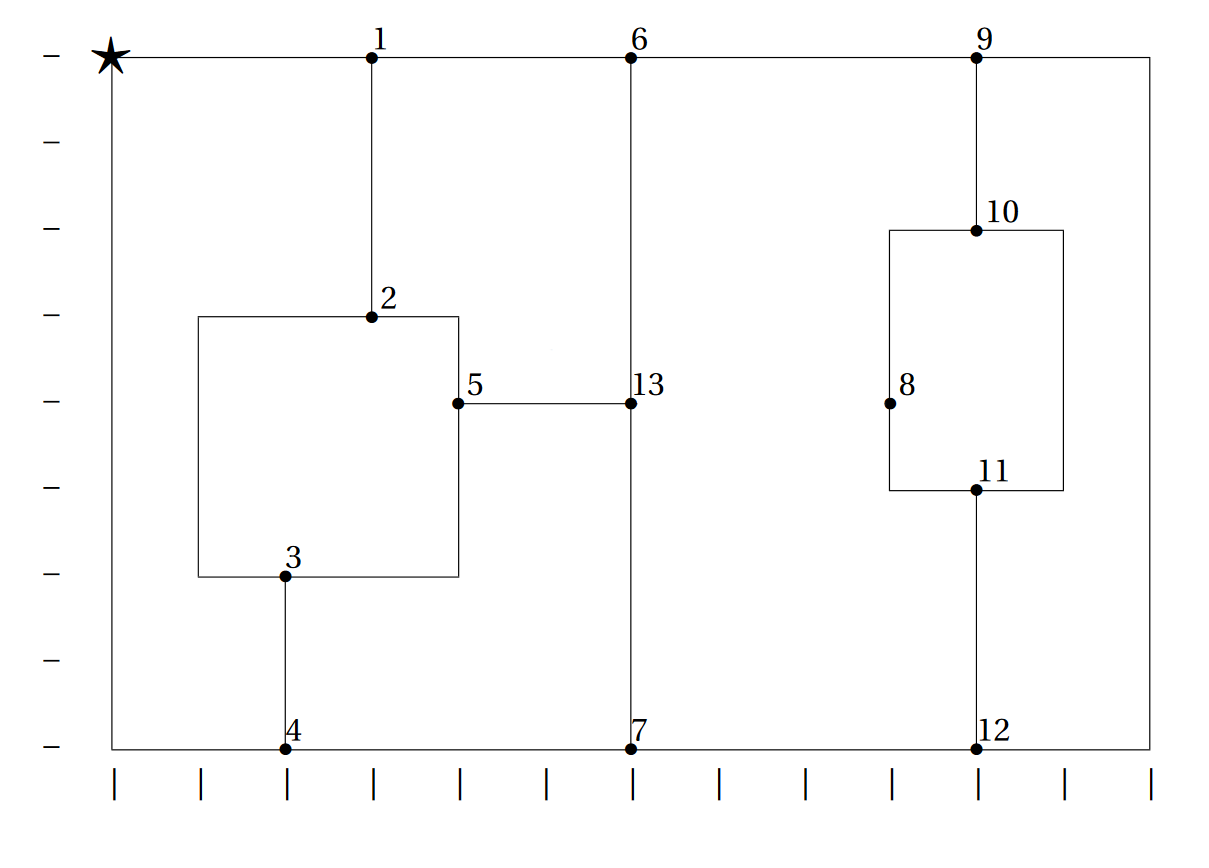
\includegraphics[width=0.8\linewidth]{fig1.png}
    \caption{Mapa de linhas de alta tensão.}
    \label{fig:mapa}
\end{figure}

Analisando com atenção o problema, chegamos à conclusão que o caminho que o nosso drone tem que percorrer deve ser um caminho Euleriano, ou mais especificamente um circuito Euleriano, pois deve começar e terminar o caminho no mesmo ponto do grafo, que neste caso é o nosso mapa. Um caminho Euleriano é um caminho de um grafo em que todas as arestas são percorridas uma única vez. Esta seria a solução ideal do nosso problema, mas, tal como diz o Teorema de Euler, apenas podemos ter um circuito Euleriano se todos os vértices do nosso grafo tiverem um grau par. Esse não é o caso no mapa que temos, logo para podermos ter um circuito Euleriano teremos que adicionar arestas ao mapa.

Chegamos desta forma ao nosso problema de otimização: \emph{que arestas é que temos que adicionar ao nosso mapa para que o caminho percorrido pelo drone seja Euleriano, e desta forma minimizar a distância total que percorre.}

Esta distância que temos de minimizar é o comprimento das arestas que iremos adicionar ao mapa, podemos ignorar o comprimento das linhas de alta tensão, pois o drone terá obrigatoriamente que as percorrer, logo esse valor será sempre constante.

Tal como referimos há pouco, para podemos ter um circuito Euleriano, todos os vértices do mapa devem ter grau par. Deste modo, as arestas a adicionar devem ligar pares de vértices de grau ímpar. Na figura seguinte assinalámos todos os vértices do nosso mapa com grau ímpar, e que teremos que ligar com arestas, que podem incidir em linhas de alta tensão ou não.

\begin{figure}[h]
    \centering
    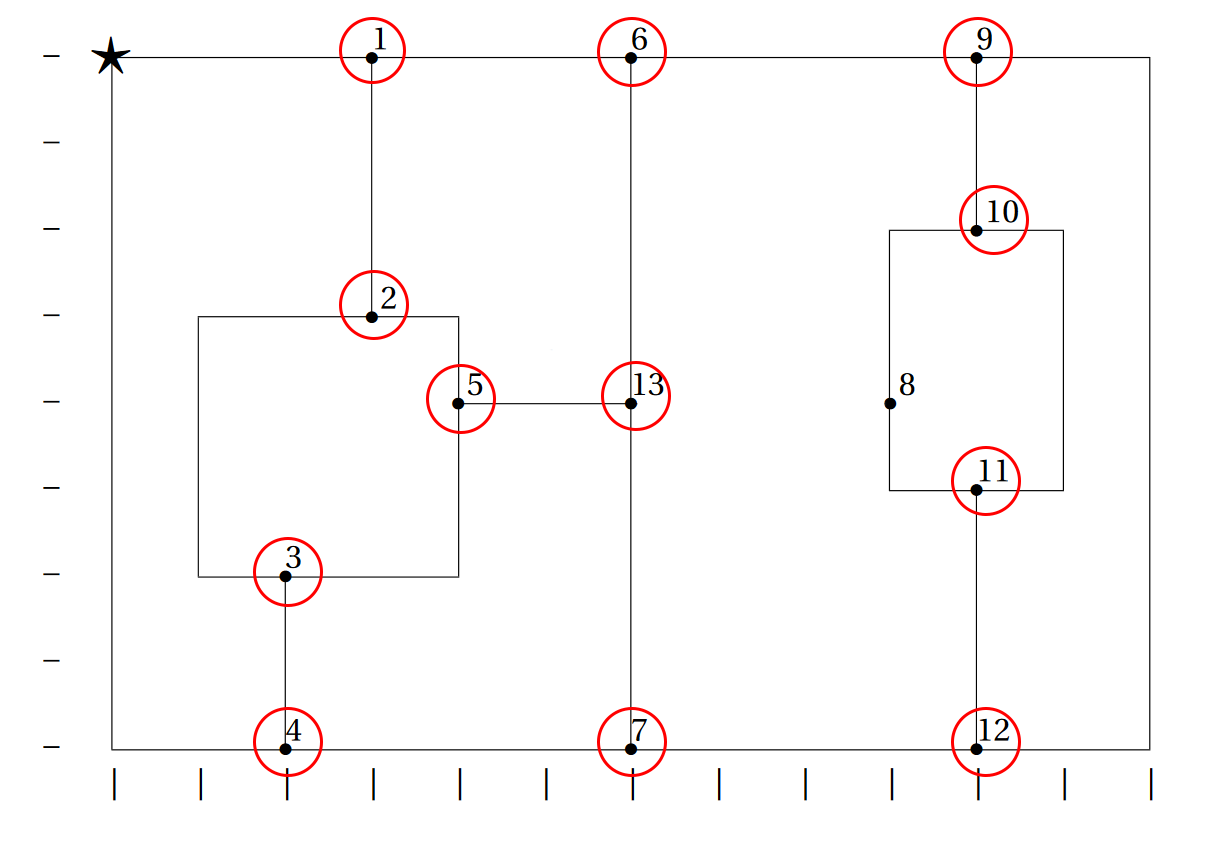
\includegraphics[width=0.8\linewidth]{fig2.png}
    \caption{Vértices de grau ímpar.}
    \label{fig:verticesimpares}
\end{figure}

Podemos ver que todos os vértices exceto o vértice 8 possuem grau ímpar, logo incluiremos todos os vértices exceto o vértice 8 no nosso modelo.

\section{Modelo}

NOTA: Decidimos usar o sistema hexadecimal (base 16) para representar os vértices nas variáveis de decisão, dado que temos mais que 10 e menos que 16 vértices, e assim podemos representar todos os vértices com apenas um dígito. Deste modo, os vértices 'a' a 'd' correspondem aos vértices 10 a 13.

Temos assim o conjunto da numeração dos vértices usados no nosso modelo definido por $ V = \{1,2,3,4,5,6,7,9,a,b,c,d\} $. Usaremos \emph{V} para nos referirmos a este conjunto de valores daqui em diante por razões de simplificação.

\subsection{Variáveis de decisão}

\(x_{ij}\): existe ou não uma aresta a unir os vértices \emph{i} e \emph{j}, $ i, j \in V, i < j $\\
\(x_{ij} \in \{ 0,1 \}\)\\

\noindent Como $ x_{ij} $ e $ x_{ji} $ representam a existência da mesma aresta, decidimos usar como variável de decisão $ x_{ij}: i < j $. Por exemplo, para representar a existência da aresta que une os vértices 5 e 9 usamos sempre $ x_{59} $ e nunca $ x_{95} $.

\subsection{Parâmetros}

$ d_{ij} $: comprimento da aresta que une os vértices \emph{i} e \emph{j}.\\
Os comprimentos de todas as arestas podem ser calculados a partir da seguinte tabela:

\begin{figure}[H]
    \centering
    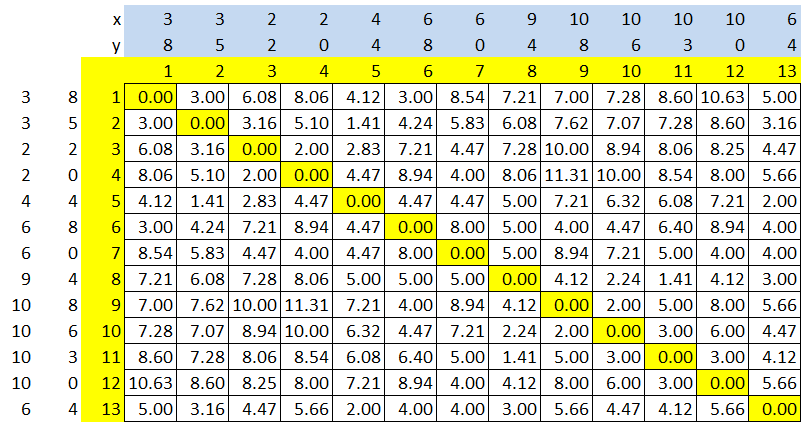
\includegraphics[width=0.8\linewidth]{fig3.png}
    \caption{Distâncias entre todos os vértices do mapa.}
    \label{fig:dists}
\end{figure}

\subsection{Função objetivo}

Minimização do comprimento das arestas a adicionar.\\
\(min: \sum_{i,j \in V} d_{ij} \times x_{ij}, i < j\)

\subsection{Restrições}

Cada vértice apenas deve fazer parte de uma aresta.\\
\(\forall i \in V: \sum x_{ij} = 1, j \in V, i < j\)

\begin{figure}[H]
    \centering
    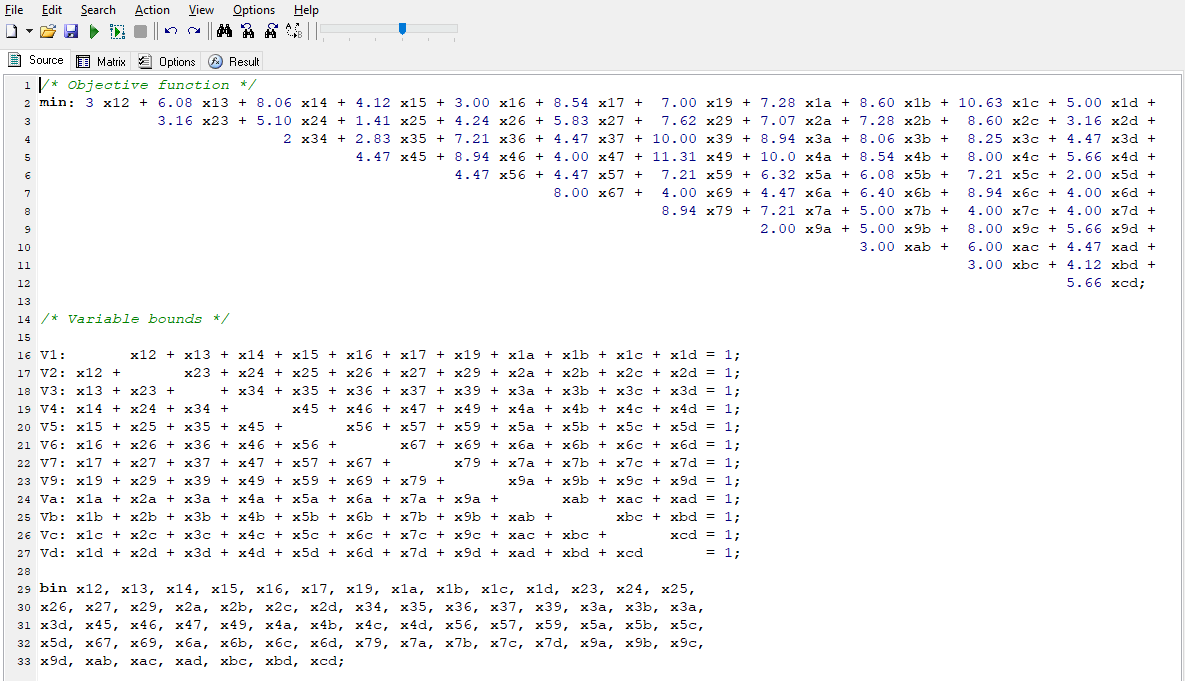
\includegraphics[width=0.8\linewidth]{lpsolve1.png}
    \caption{Ficheiro de input no LPSolve IDE.}
    \label{fig:lp}
\end{figure}

\section{Solução ótima}

Depois de introduzir o modelo do problema no \emph{LPSolve}, chegamos a uma aparente solução ótima, onde são criadas arestas a unir os vértices 1 ao 6, o 2 ao 5, o 3 ao 4, o 7 ao 13, o 9 ao 10 e o 11 ao 12, com um comprimento total de 15,41. 

\begin{figure}[H]
    \centering
    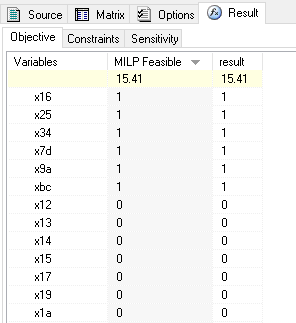
\includegraphics[width=0.4\linewidth]{lpsolve2.png}
    \caption{Output produzido pelo LPSolve IDE.}
    \label{fig:lpoutput}
\end{figure}

A seguinte figura ilustra esta solução: 

\begin{figure}[H]
    \centering
    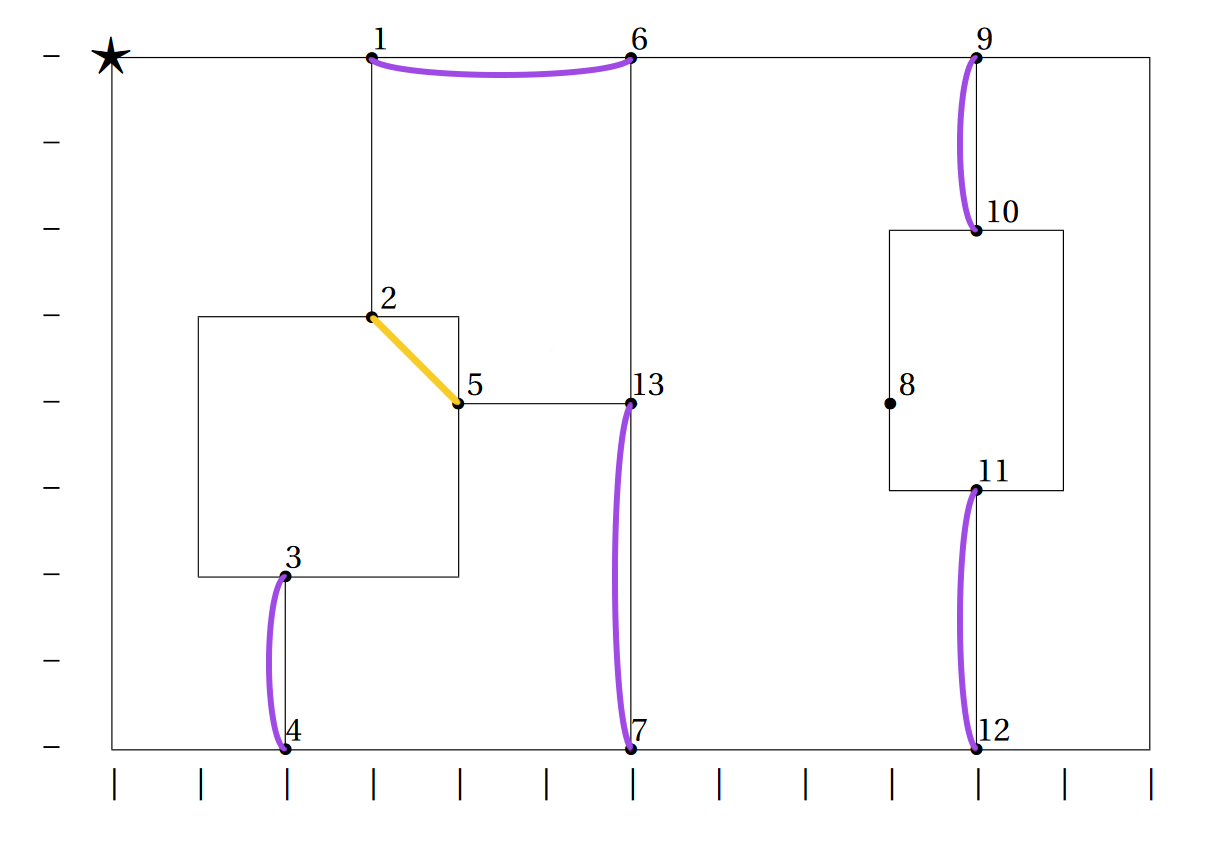
\includegraphics[width=0.8\linewidth]{fig4.png}
    \caption{Arestas a adicionar ao grafo.}
    \label{fig:arestas}
\end{figure}

As arestas roxas indicam que o drone terá que percorrer as linhas de alta tensão correspondentes duas vezes, e a aresta amarela indica uma distância que o drone percorrerá pelo ar. Desta forma já temos um grafo onde todos os vértices têm grau par, e podemos então definir um circuito Euleriano para o drone. Visto que o circuito terá que passar por todas as arestas exatamente uma vez, a distância total percorrida pelo drone será sempre a mesma, e não é necessário minimizar esta distância total. Portanto, apenas nos falta desenhar o trajeto do drone. Temos várias possibilidades para este trajeto, por isso iremos apenas apresentar um exemplo:

\begin{figure}[H]
    \centering
    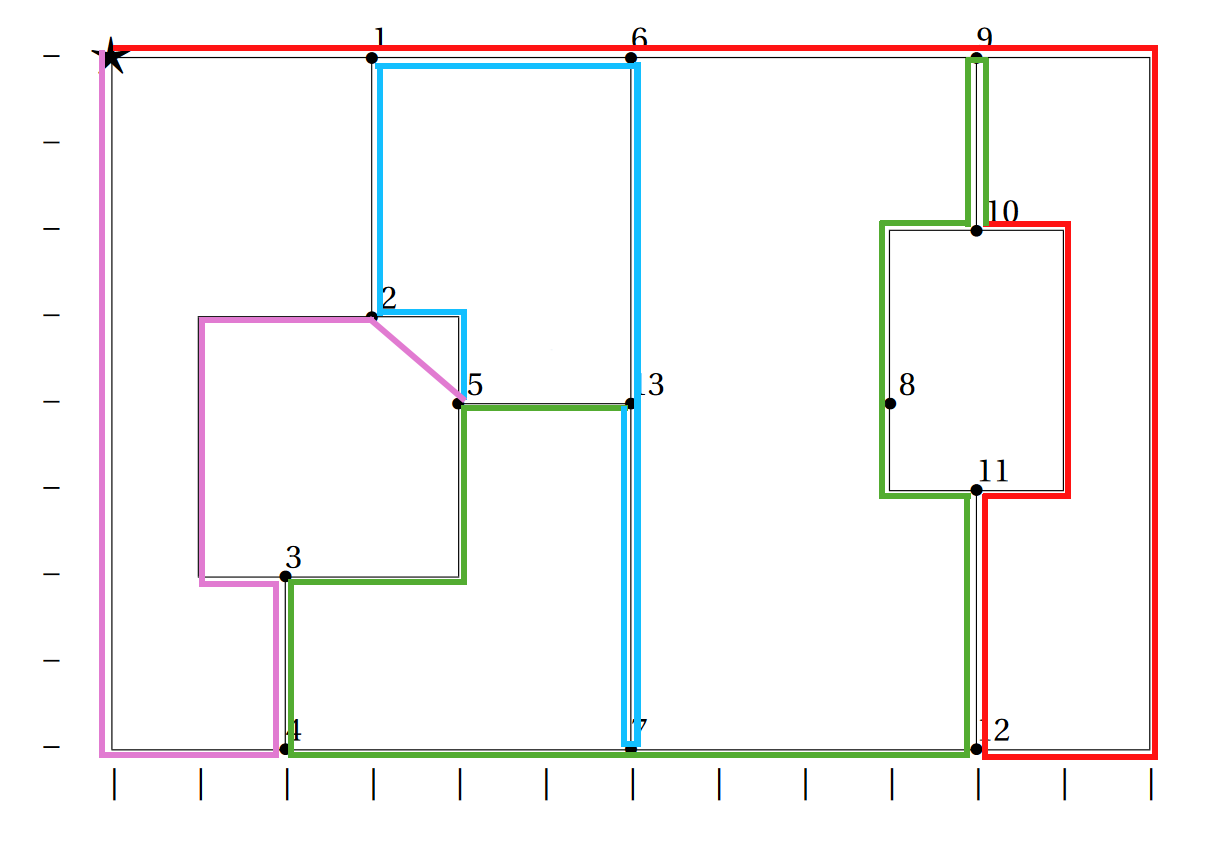
\includegraphics[width=0.8\linewidth]{fig5.png}
    \caption{Possível solução do problema.}
    \label{fig:solucao}
\end{figure}

Dentro desta solução temos dois possíveis percursos. No primeiro o drone percorre a linha vermelha, depois a linha verde, depois a linha azul e por fim a linha rosa. O outro percurso possível é o inverso deste.

Seja qual for o percurso que definirmos a partir deste mapa, a distância total percorrida pelo drone será sempre a soma dos comprimentos das linhas de alta tensão com o comprimento das arestas que adicionámos, ou seja, 82 + 15,41 = 97,41.

\section{Validação do modelo}

A seguinte tabela ilustra as restrições do nosso modelo, e tal como podemos observar, todas as restrições são cumpridas, para cada vértice de grau ímpar apenas criamos uma aresta. 

\begin{figure}[H]
    \centering
    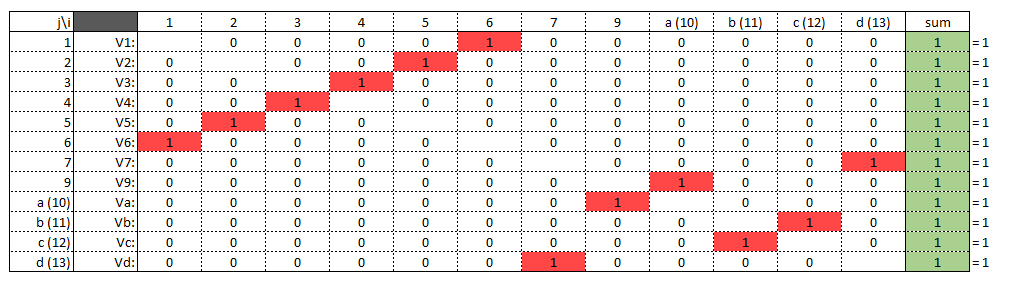
\includegraphics[width=0.8\linewidth]{fig6.png}
    \caption{As restrições são todas cumpridas.}
    \label{fig:restricoes}
\end{figure}

Hipoteticamente também poderia existir uma solução onde adicionávamos mais que uma aresta por vértice, desde que os vértices permanecessem com grau par continuaria a ser uma solução válida, mas não seria ótima. Para o provar voltámos a correr o nosso modelo no LPSolve, mas trocando o '=' das restrições por '>=', e como agora podemos adicionar mais que um vértice a cada aresta devemos também adicionar o vértice 8. Isto não garante que todos os vértices passem a ser de grau par, mas o que queremos comprovar com este exemplo é que a solução obtida anteriormente é ótima, e é precisamente isso que concluímos, pois o resultado deste novo modelo é exatamente o mesmo. Isto significa que, mesmo que pudéssemos adicionar mais que uma aresta a cada vértice, na solução ideal continuaríamos a adicionar apenas um, logo a nossa restrição no modelo original é válida.

\begin{figure}[H]
    \centering
    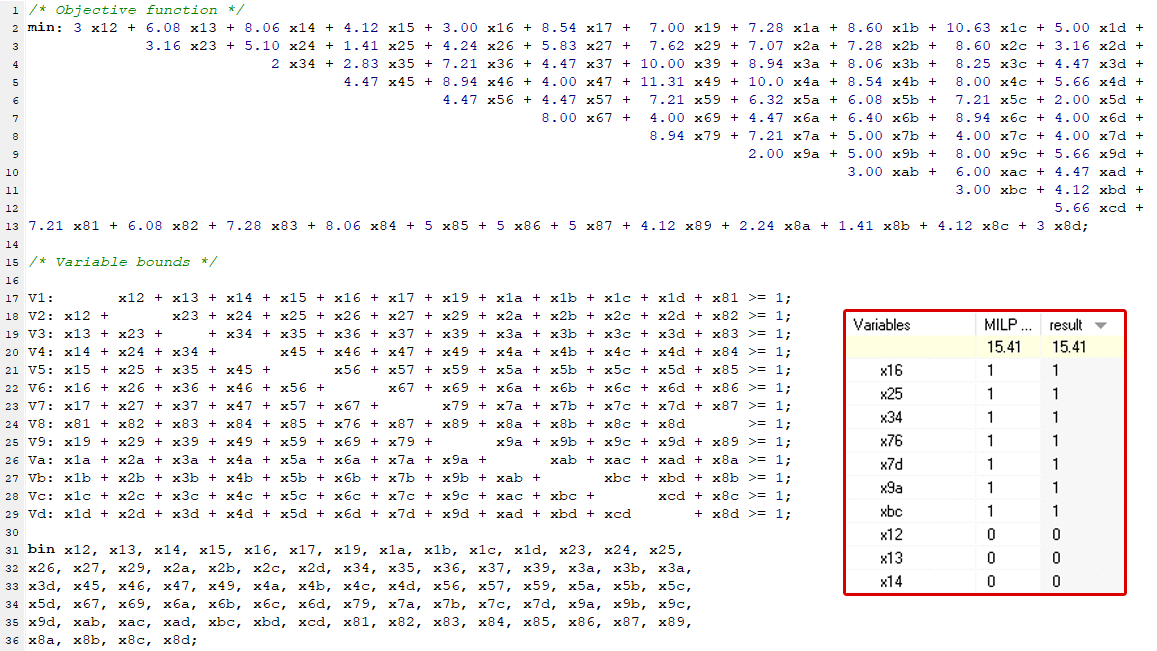
\includegraphics[width=0.9\linewidth]{fig7.png}
    \caption{Modelo alternativo, onde podemos ligar mais que uma aresta a cada vértice, e respetiva solução.}
    \label{fig:altmodelo}
\end{figure}

\end{document}